\documentclass[11pt]{amsart}
\usepackage[a4paper,textwidth=158mm,textheight=237mm,centering]{geometry}
\usepackage[T1]{fontenc}
\usepackage{lmodern,microtype,mathtools,amssymb,graphicx,flafter}
\usepackage[unicode,colorlinks=true,linkcolor=black,citecolor=black,urlcolor=blue]{hyperref}
\newtheorem{theorem}{Theorem}
\newcommand{\av}[1]{\left\langle #1\right\rangle}
\newcommand{\rev}[1]{\overline{#1}}
\title[A periodic waiting-time counterexample]{A counterexample to a periodic waiting-time entropy bound}
\author{Harvey Yorke}\address{Valyu AI}
\ifdefined\journalversion
\hypersetup{pdfauthor={Harvey Yorke}}
\else
\author{Valyu DeepResearch}\address{Valyu AI}
\hypersetup{pdfauthor={Harvey Yorke and Valyu DeepResearch}}
\fi
\hypersetup{pdftitle={A counterexample to a periodic waiting-time entropy bound}}
\date{18 October 2026}
\newcommand{\paperAuthorBlock}[1]{%
  \begin{minipage}[t]{.44\textwidth}\centering\normalfont\normalsize
  #1\par\small Valyu AI\par\end{minipage}}
\makeatletter
\renewcommand{\@setauthors}{%
  \begingroup\trivlist\centering\normalfont\normalsize
  \@topsep30\p@\relax\advance\@topsep by -\baselineskip\item\relax
  \ifdefined\journalversion\paperAuthorBlock{Harvey Yorke}%
  \else\paperAuthorBlock{Harvey Yorke}\hspace{.06\textwidth}%
  \paperAuthorBlock{Valyu DeepResearch}\fi\endtrivlist\endgroup}
\renewcommand{\@setaddresses}{}
\makeatother
\begin{document}
\raggedbottom
\begin{abstract}
Maier, Deg\"unther, van der Meer and Seifert conjectured that a waiting-time
estimator constructed entirely from the forward protocol bounds the entropy
production of a periodically driven Markov network from below.
We give an analytic three-state counterexample. The two observed links have
symmetric rates $1+\varepsilon\cos t$ and $1+\varepsilon\sin t$, and the
hidden link has constant symmetric rate one, with $0<\varepsilon<1$.
The stationary distribution remains uniform and the defined Markov entropy
production is identically zero. Nevertheless, two reversed event-pair
waiting densities have derivative difference $\varepsilon^2$ at zero lag,
making the estimator strictly positive. All rates are smooth and uniformly
positive. The result concerns the forward-protocol conjecture, not the
separate theorem using data from the time-reversed protocol.
\end{abstract}
\maketitle
\begin{center}\small
Research draft. Exact checks and internal proof reviews are available;
author approval, priority assessment and external review remain open.
\end{center}

\section{The conjectured bound}
Consider a continuous-time Markov chain with periodically driven rates
$k_{ij}(t)$, period $T$, and periodic stationary distribution $p_i(t)$.
An observer records a reversal-closed set $\mathcal L$ of directed jump
labels. Write $\rev I$ for the label with opposite direction and
$\bar n_I$ for the mean occurrence rate of label $I$.
Let $\Psi_{I\to J}(s)$ be the joint density that the next observed label is
$J$ and that its delay after an event $I$ is $s$, averaged over the phase
distribution of occurrences of $I$. Thus
\begin{equation}\label{eq:rownorm}
 \sum_{J\in\mathcal L}\int_0^\infty\Psi_{I\to J}(s)\,ds=1.
\end{equation}
Individual label-pair densities need not have unit integral.

Maier et al.\ propose the estimator \cite{maier2024}
\begin{equation}\label{eq:estimator}
 \widehat\sigma_\Psi=
 \sum_{I,J\in\mathcal L}\bar n_I\int_0^\infty
 \Psi_{I\to J}(s)
 \log\frac{\Psi_{I\to J}(s)}{\Psi_{\rev J\to\rev I}(s)}\,ds
\end{equation}
and conjecture $0\leq\widehat\sigma_\Psi\leq\bar\sigma$, where
\begin{equation}\label{eq:ep}
 \bar\sigma=\frac1T\int_0^T\sum_{i,j}
 p_i(t)k_{ij}(t)\log\frac{p_i(t)k_{ij}(t)}{p_j(t)k_{ji}(t)}\,dt.
\end{equation}
These are Eqs.\ (17), (18), and (3), respectively, of the published article;
they correspond to Eqs.\ (14), (15), and (3) of arXiv:2406.12657v1.
Crucially, both waiting densities in \eqref{eq:estimator} are measured
under the \emph{same forward protocol}. Only the event labels reverse.
The source distinguishes this conjecture from its proved Eq.\ (16)
(arXiv-v1 Eq.\ (13)), which uses data generated by the reversed protocol.

The published general setup imposes periodic rates and local detailed
balance, with no restriction to constant symmetric kinetic prefactors.
The counterexample below changes symmetric kinetic rates while keeping
all local free-energy differences and affinities zero.

\section{A smooth three-state counterexample}
Use time units in which the hidden rate and driving angular frequency
are both one. Take $T=2\pi$, $0<\varepsilon<1$, and set
\begin{align}\label{eq:rates}
 k_{12}(t)=k_{21}(t)&=a(t)=1+\varepsilon\cos t,\nonumber\\
 k_{23}(t)=k_{32}(t)&=b(t)=1+\varepsilon\sin t,\\
 k_{13}(t)=k_{31}(t)&=1.\nonumber
\end{align}
Observe $\mathcal L=\{12,21,23,32\}$ and leave the edge $13$ hidden.
All states are ordinary states even under time reversal.

\begin{theorem}\label{thm:counterexample}
For every $0<\varepsilon<1$, the network \eqref{eq:rates} has
\[
 \bar\sigma=0<\widehat\sigma_\Psi<\infty.
\]
Consequently the upper inequality in the forward-protocol conjecture
fails for smooth, strictly positive, periodically driven Markov rates.
\end{theorem}

\begin{proof}
Every instantaneous generator is symmetric. Hence
$p_1(t)=p_2(t)=p_3(t)=1/3$ is the periodic stationary distribution,
and each summand in \eqref{eq:ep} is zero. Positivity of all rates
ensures uniqueness of this periodic distribution. The rate ratios are
one, satisfying local detailed balance with zero free-energy differences
and zero affinities.

Write $\av{q}=(2\pi)^{-1}\int_0^{2\pi}q(t)\,dt$. Since
$\av a=\av b=1$, each observed directed event has mean rate
$\bar n_I=1/3$. Conditional on the occurrence of $12$, the phase density
is $a(t)/(2\pi)$; conditional on $32$, it is $b(t)/(2\pi)$.
This event weighting is essential.

After either event the system occupies state $2$, whose exits are both
observed. Define
\begin{equation}\label{eq:survival}
 H(t,s)=\int_t^{t+s}(a(u)+b(u))\,du.
\end{equation}
The two reversed label-pair densities are therefore exactly
\begin{align}\label{eq:fg}
 f(s):=\Psi_{12\to23}(s)&=\av{a(t)b(t+s)e^{-H(t,s)}},\nonumber\\
 g(s):=\Psi_{32\to21}(s)&=\av{b(t)a(t+s)e^{-H(t,s)}}.
\end{align}
They satisfy $f(0)=g(0)=\av{ab}=1$.
Differentiation under the phase integral is justified by smoothness
on a compact domain. The two survival derivatives cancel, leaving
\begin{align}\label{eq:derivative}
 (f-g)'(0)&=\av{ab'-ba'}\nonumber\\
 &=\av{\varepsilon\cos t+\varepsilon\sin t+\varepsilon^2}
 =\varepsilon^2>0.
\end{align}
Thus $f(s)>g(s)>0$ on a nonempty interval of positive delays.

Every state has an observed exit rate at least $1-\varepsilon$.
The survival probability of no observed event for a delay $s$ is at most
$e^{-(1-\varepsilon)s}$, proving \eqref{eq:rownorm}. On the product
space of label pairs and positive delays, define probability densities
\[
 P(I,J,s)=\tfrac14\Psi_{I\to J}(s),\qquad
 Q(I,J,s)=\tfrac14\Psi_{\rev J\to\rev I}(s).
\]
Both integrate to one because reversal permutes the label pairs.
Equal event rates give the exact identity
\begin{equation}\label{eq:kl}
 \widehat\sigma_\Psi=\frac43 D_{\mathrm{KL}}(P\Vert Q)>0.
\end{equation}
Strictness follows from \eqref{eq:derivative}, since $P\ne Q$ on a
set of positive measure.

For completeness, the divergence is finite. From state $2$, the only
possible next labels are $21$ and $23$. From states $1$ or $3$, the
only hidden evolution is a rate-one symmetric chain on $\{1,3\}$,
and the next labels are $12$ or $32$. The allowed pair set is invariant
under reversal. The hidden chain's transition probabilities are
$(1\pm e^{-2s})/2$, according to whether its endpoints agree.
The survival weighting multiplies these probabilities by a factor
between $e^{-(1+\varepsilon)s}$ and $e^{-(1-\varepsilon)s}$.
Put $\delta=1-\varepsilon$ and $b_*=1+\varepsilon$.
Initial phase and final event-rate factors give, for a pair with hidden
endpoint transition probability $q_s=(1\pm e^{-2s})/2$,
\[
 \delta^2 e^{-b_*s}q_s\leq\Psi_{I\to J}(s)
       \leq b_*^2 e^{-\delta s}q_s.
\]
Reversal preserves the hidden endpoint parity, so $q_s$ cancels in
the density ratio. For state-$2$ pairs, \eqref{eq:survival} gives the
same bounds with $q_s=1$ and doubled decay exponents. Consequently every
allowed pair satisfies
\[
 \left|\log\frac{\Psi_{I\to J}(s)}
 {\Psi_{\rev J\to\rev I}(s)}\right|
 \leq 2\log(b_*/\delta)+4\varepsilon s.
\]
The densities are bounded by $b_*^2e^{-\delta s}$, proving integrability.
Impossible pairs vanish in both densities and contribute zero.
\end{proof}

\begin{figure}[ht]
 \centering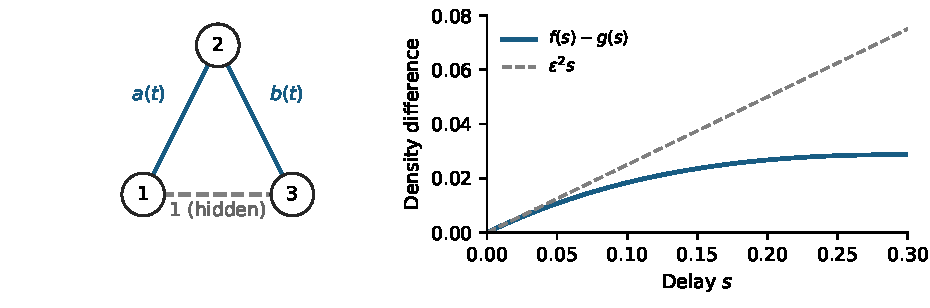
\includegraphics[width=\textwidth]{counterexample.pdf}
 \caption{Left: the two observed links have symmetric rates $a(t)$ and
 $b(t)$; the dashed hidden link has symmetric rate one. Right: the
 difference $f(s)-g(s)$ at $\varepsilon=1/2$ and its exact tangent
 $\varepsilon^2s$ at zero. Periodic quadrature illustrates the densities;
 the proof uses the analytic identity \eqref{eq:derivative}.}
 \label{fig:model}
\end{figure}

\section{Interpretation, prior context, and verification}
The nonzero estimate records the temporal ordering of kinetic rates.
It does not require a probability current: in this family every
instantaneous current and every term in \eqref{eq:ep} vanish.
More generally, for positive smooth functions $a,b$ with common mean
$m$, the same construction gives
\[
 (f-g)'(0)=\frac{\av{ab'-ba'}}{m}.
\]
A nonzero signed area enclosed by the periodic rate-plane curve
therefore supplies a sufficient condition for this waiting-time
asymmetry. This geometric observation explains the mechanism rather
than asserting a new general relation between time asymmetry and
dissipation.

Waiting-time irreversibility at equilibrium is already known.
Hartich and Godec give an equilibrium counterexample based on hidden
transitions and explain its kinetic-hysteresis interpretation
\cite{hartich2021}. Our construction observes actual directed edges;
its asymmetry comes from marginalizing the driving phase while
retaining the forward protocol in both comparison laws.
It is not the first waiting-time false positive.

Protocol reversal is already central to the source's proved bound.
Harunari, Fiore and Barato independently study periodically driven
waiting-time inference, explicitly use reversed-protocol distributions,
and discuss Maier et al.'s forward-protocol proposal as a conjecture
\cite{harunari2024}. Their kinetic-barrier models are close prior context.
The result here is the explicit failure of the stated forward-protocol
upper bound. Neither reversed-protocol result is contradicted.

There is also no assertion that a physical autonomous device generating
the protocol dissipates no energy. Such a controller is absent from
\eqref{eq:ep}. The theorem concerns precisely the Markov entropy
production used in the conjecture. It does not identify the total
thermodynamic cost of implementing time-dependent rates.

The proof requires no trajectory simulation or parameter search.
An independent exact Fourier-polynomial calculation over the rationals
verifies
\[
 f'(0)=-2-\tfrac12\varepsilon^2,\qquad
 g'(0)=-2-\tfrac32\varepsilon^2.
\]
From this directory, the command
\begin{center}\small
 \verb|python3 -B -O verification/check_short_lag.py|
\end{center}
replays these identities using the Python standard library.
\texttt{sh build.sh} runs that check and builds both author presentations;
\path{plot_counterexample.py} reproduces the illustration.
The exact checker covers the polynomial identities, while the event
conditioning, normalization, support, and integrability arguments are
proved above and recorded in the separate independent audit.
Bounded prior searches and a focused literature review are retained with
the working files. They do not establish exhaustive priority.

\ifdefined\journalversion
\section*{Research assistance}
Valyu DeepResearch supported literature retrieval and source comparison.
Coding agents developed the counterexample and analytic
argument, implemented the exact verification program, and drafted and
revised the manuscript. The exact checks cover the stated Fourier
identities; they do not formalize the probability argument or constitute
external peer review.
\fi

\bibliographystyle{plain}
\bibliography{references}
\end{document}
